\chapter{Munich WAN}

\section{Site Overview}
Munich is the other branch of the RECOMP Corporation. The network has:
\begin{itemize}
    \item Two Routers (2911 model);
    \item Four switch Layer 2 switches (2960-24TT model);
    \item Four PCs representing each of the networks present in each branch: Staff, Accounting, Human Resources and Users.
\end{itemize}

The topology of the Munich branch is shown in Figure \ref{fig:munichtopology}. The Munich \ac{WAN} is connected to the Internet using the address block 193.136.60.147/29.


\begin{figure}[!htb]
\centering
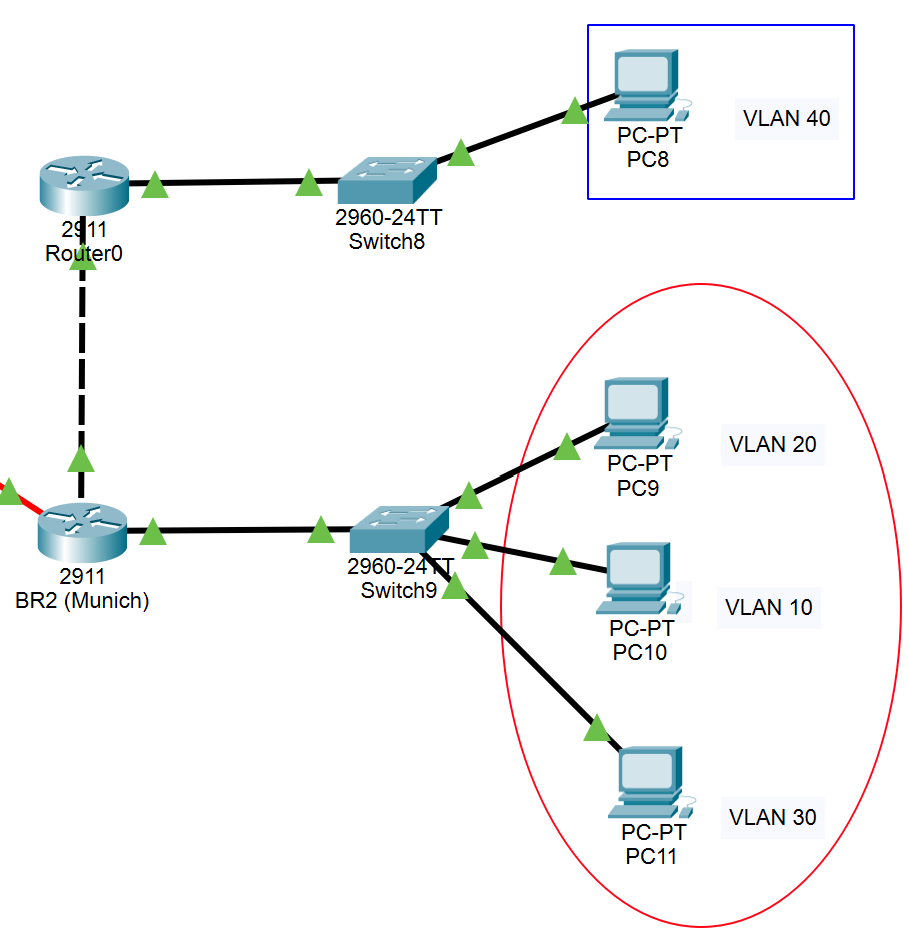
\includegraphics[width=0.6\textwidth]{figures/munich_topology.png}
\caption{\label{fig:munichtopology}Munich WAN Topology}
\end{figure}

\section{Munich WAN Addressing}

\begin{center}
\setlength{\LTleft}{-1.5cm}
\begin{longtable}{
|>{\centering\arraybackslash}p{3cm}|
 >{\centering\arraybackslash}p{2cm}|
 >{\centering\arraybackslash}p{3cm}|
 >{\centering\arraybackslash}p{2.5cm}|
 >{\centering\arraybackslash}p{1cm}|
 >{\centering\arraybackslash}p{5cm}|}
\hline
\textbf{Networks} & 
\textbf{Number of Nodes} & 
\textbf{Network Address} & 
\textbf{Broadcast} & 
\textbf{Mask} & 
\textbf{First and Last Hosts} \\ \hline
\endfirsthead

\hline
\textbf{Networks} & 
\textbf{Number of Nodes} & 
\textbf{Network Address} & 
\textbf{Broadcast} & 
\textbf{Mask} & 
\textbf{First and Last Hosts} \\ \hline
\endhead

USERS & 200 & 172.18.78.0 & 172.18.78.255 & /24 & 172.18.78.1 -- 172.18.78.254 \\ \hline
ACCOUNTING & 20 & 172.18.79.0 & 172.18.79.31 & /27 & 172.18.79.1 -- 172.18.79.30 \\ \hline
STAFF & 10 & 172.18.79.32 & 172.18.79.47 & /28 & 172.18.79.33 -- 172.18.79.46 \\ \hline
HR & 10 & 172.18.79.48 & 172.18.79.63 & /28 & 172.18.79.49 -- 172.18.79.62 \\ \hline


\caption{Munich Addressing}
\end{longtable}
\end{center}


\section{Implementation of Cisco Commands}

In this Munich branch, the goal was to implement VLAN segmentation, inter-VLAN routing, DHCP address allocation and connectivity between remote sites through static routing.

\subsection*{Switch Configuration}

The Switch7 (SW7), was configured to handle three departments: Staff, Accounting, and Human Resources (HR).
The following VLANs were created:

\begin{lstlisting}[caption={VLAN creation on SW7}, label={lst:sw7-vlan-creation}]
vlan 10
  name STAFF
vlan 20
  name ACCOUNTING
vlan 30
  name HR
vlan 50
  name NATIVE
vlan 99
  name BLACKHOLE
\end{lstlisting}

The trunk link connecting SW7 to router BR2 was configured on the \textit{gigabitEthernet0/1} interface, allowing VLANs 10, 20 and 30 and using VLAN 50 as the native VLAN:

\begin{lstlisting}[caption={Trunk configuration on SW7}, label={lst:sw7-trunk}]
interface gigabitEthernet0/1
    switchport mode trunk
    switchport trunk native vlan 50
    switchport trunk allowed vlan 10,20,30
\end{lstlisting}

The access ports for the end-user PCs were then assigned to their respective VLANs.

\begin{lstlisting}[caption={Access port configuration on SW7}, label={lst:sw7-access}]
interface range fa0/1-5
    switchport mode access
    switchport access vlan 10
    no shutdown
exit

interface range fa0/6-10
    switchport mode access
    switchport access vlan 20
    no shutdown
exit

interface range fa0/11-15
    switchport mode access
    switchport access vlan 30
    no shutdown
exit

interface range fa0/16-24
    switchport mode access
    switchport access vlan 99
    shutdown
\end{lstlisting}

The ports not used were assigned to Blackhole VLAN 99 and administratively shutdown to improve security.

Switch8 (SW8), used for local users in Users VLAN 40, was configured with VLAN 40, 50 and 99:

\begin{lstlisting}[caption={VLAN creation on SW8}, label={lst:sw8-vlan-creation}]
vlan 40
  name USERS
vlan 50
  name NATIVE
vlan 99
  name BLACKHOLE
\end{lstlisting}


Secondly, we configured many different network interfaces for vlan 40 and vlan 99:

\begin{lstlisting}[caption={Access port configuration on SW8}, label={lst:sw8-access}]
interface range fa0/1-24
    switchport mode access
    switchport access vlan 40
    no shutdown
exit

interface range gigabitEthernet0/2
    switchport mode access
    switchport access vlan 99
    shutdown
exit    
\end{lstlisting}

\subsection*{Router Configuration}

\subsection*{DHCP Configuration}

\subsection*{* Configuration}

\subsection*{* Configuration}